\normaltrue \difficilefalse \tdifficilefalse
\correctiontrue

%\UPSTIidClasse{11} % 11 sup, 12 spé
%\newcommand{\UPSTIidClasse}{11}

\exer{Calcul de FTBO$\star$ \label{B2:07:505}}
\setcounter{question}{0}\marginnote{\xpComp{SLCI}{03}}%\UPSTIcompetence{B2-07}
\index{Compétence B2-07}\index{Compétence SLCI-03}
\index{Schéma-blocs}
\index{FTBO}

\ifcorrection
\else
\marginnote{\textbf{Pas de corrigé pour cet exercice.}}
\fi


\question{Déterminer la FTBO dans la cas suivant.}
\ifprof 
$FTBO(p) = A(p) B(p) C(p)$.
\else
\begin{marginfigure}
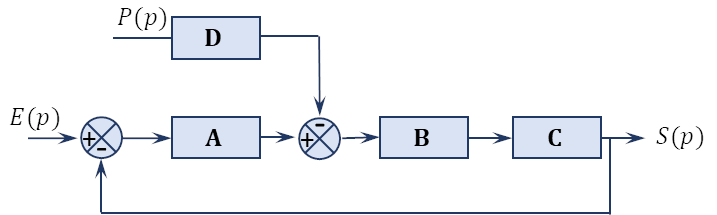
\includegraphics[width=\linewidth]{512_01}
\end{marginfigure}
\fi
 
\question{Déterminer la FTBO dans la cas suivant.}

\ifprof 
$FTBO(p) = B(p) C(p)$.
\else
\begin{marginfigure}
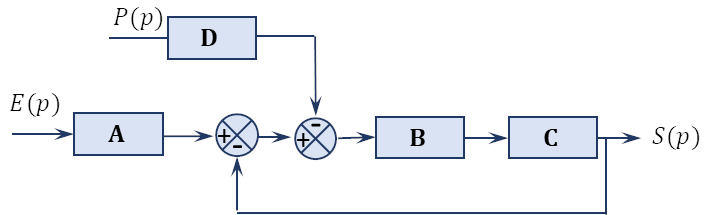
\includegraphics[width=\linewidth]{512_02}
\end{marginfigure}
\fi

\question{Déterminer la FTBO dans la cas suivant.}

\ifprof 
$FTBO(p) = B(p) C(p)$.
\else
\begin{marginfigure}
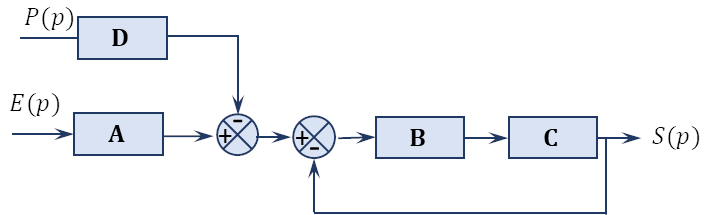
\includegraphics[width=\linewidth]{512_03}
\end{marginfigure}
\fi

\question{Déterminer la FTBO dans la cas suivant.}

\ifprof 
$ FTBO(p) = \dfrac{B(p) C(p)}{1+B(p) C(p) E(p)} \times \dfrac{A(p) D(p)}{C(p)}$ 
\else
\begin{marginfigure}
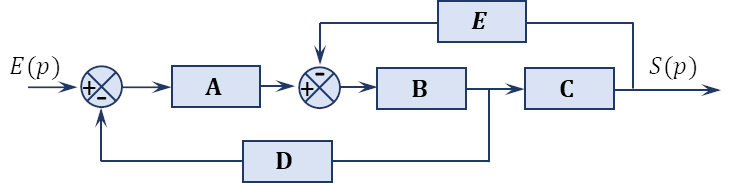
\includegraphics[width=\linewidth]{512_04}
\end{marginfigure}
\fi



%\question{Réaliser le schéma-blocs.}
%\ifprof
%\begin{marginfigure}
%\centering
%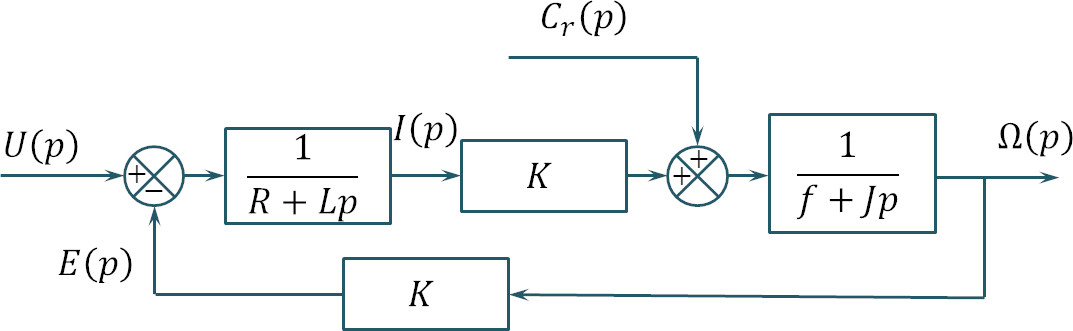
\includegraphics[width=\linewidth]{51_01_c}
%%\caption{Évolution du couple utile en fonction de la vitesse de rotation pour des
%%fréquences de commande de \SI{90}{Hz} à \SI{110}{Hz}. \label{fig_50_04}}
%\end{marginfigure}
%\else
%\fi



\ifprof
\else
\marginnote{Corrigé voir \ref{B2:07:505}.}
\begin{solution}
\begin{enumerate}
\item $FTBO(p) = A(p) B(p) C(p)$.
\item $FTBO(p) = B(p) C(p)$.
\item $FTBO(p) = B(p) C(p)$.
\item $FTBO(p) = \dfrac{B(p) C(p)}{1+B(p) C(p) E(p)} \times \dfrac{A(p) D(p)}{C(p)}$.
\end{enumerate}
\end{solution}

\fi